\documentclass[a4paper,12pt]{article}

\RequirePackage{epsfig}

\setlength\hoffset{-0.5in}      %% these work quite well with a 12pt font
\setlength\voffset{-0.5in}
\setlength{\textwidth}{6.30in}
\setlength{\textheight}{9.0in}

\usepackage{longtable}
\usepackage{array}
\usepackage{graphicx}
\usepackage{float}
\usepackage{enumitem}
\usepackage{hyperref}
\graphicspath{ {./img/} }

\bibliographystyle{unsrt}
\begin{document}

\begin{center}
{\Large\bf{Decentralised Blockchain Security Architecture for IoT and MQTT Brokers}} \\
      \vspace{5.0mm}
{\Large\bf{Project Plan}} \\
      \vspace{8mm}
      {\large\bf{Konrad Dryja}}  \\
      \vspace{5.0mm}
       {\tt k.dryja.15@abdn.ac.uk} \\
      \vspace{5.0mm}
      {\em Department of Computing Science,\\
       University of Aberdeen, Aberdeen AB24 3UE, UK} 
\end{center}


\section*{Introduction}

Internet of Things (further referred as IoT) is a growing field concerning interconnectivity of various smart devices. Equipment such as smart bus timetables, doorbells, thermostats or even pacemakers capable of sending alerts directly to emergency services are omnipresent. It's a system of computers, chips, phones, sensors deployed in our lives that are communicating with each other without requiring any human intervention.

Sensitive personal data (as defined by GDPR\cite{EUdataregulations2018}, for example, health information) is very often handled and leak or misrepresentation can have consequences such as fines or other penalties. Additionally, IoT devices have limited computation power, which is sacrificed in favour of extended lifespan to avoid frequent maintenance, battery replacement and significantly lower initial costs. This makes it a very lucrative target for malicious actors. For example, researchers from University of Michigan performed a demo attack on a pacemaker, extracting personal information and changing the configuration\cite{4531149}.
%This example and more clearly presents a need for solution capable of securing and closing off access to unwanted agents.

What is more, those devices frequently do not directly communicate on a peer-to-peer basis, but instead pass through intermediary resource handling the distribution of data. MQTT Brokers\footnote{\url{https://mqtt.org/}} are one of them, providing a Publisher/Subscriber architecture, allowing for information exchange without the constant need of interconnectivity between clients, instead of relying on created topics used as a relay. It's very important to point out that MQTT is not a piece of software, but rather a standard describing the operation of such backend and leaves the implementation up to end-users - the implementation is very often referred as MQTT Brokers.

The documentation also clearly states that the security is not part of the standard, but rather leaves this decision up to the implementors\footnote{\url{https://docs.oasis-open.org/mqtt/mqtt/v5.0/os/mqtt-v5.0-os.html\#\_Toc3901261}}. And while the transport of data can be assumed to remain secure (as MQTT operates over TCP/IP, thus encrypting the data using TLS), the access is often not. For example, an attack could be conducted, where malicious device communicates with the broker, impersonating another IoT hardware, in process registering for secure topic (e.g. where heart rate is being published by the smart pacemaker, normally restricted only for health authorities) and intercepting the data.

\begin{figure}[ht]
  \centering
  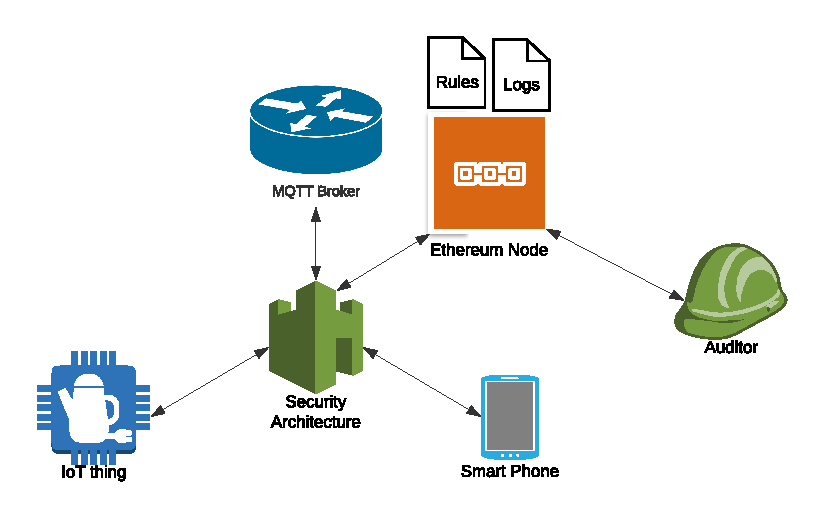
\includegraphics[scale=1.1]{iot_attack}
  \caption{Proposed architecture}\label{fig:iot1}
\end{figure}

Common implementation of MQTT brokers includes basic authentication based on a username and a secret password, offering limited to no logging or auditing of operations performed on the broker. For example, one of the most popular brokers Mosquitto\footnote{\url{https://mosquitto.org/man/mosquitto-conf-5.html}}, as of version 1.6.8 offers password based authentication with ACL capabilities restricting some credentials only to given topics. 

I would like to propose a generic, pluggable module following the description of MQTT standard (and thus potentially making it independent from the used MQTT Broker) handling Authentication, Authorization and Accountability of clients attempting connection to the brokers. In order to make the platform more resilient and independent from single points of failure (often being the central ACL repository), I will deploy it on a blockchain - which by convention supports recording of transactions (by placing them on the blockchain) and authentication via ID of the presented wallet. Figure \ref{fig:iot1} represents sketch of the proposed architecture, where the Security element would handle all incoming connections and proxy them accordingly. Due to the public nature of blockchain architecture, transactions would also be available to view by third parties for the purposes of auditing and transparency.

As mentioned, logging, auditing and accountability will be the main focus of the project. Normally, recording of every operation performed on the platform would be impractical and not scale very well, as the number of published messages sometimes can hit 100, 1000 or even more per second. Relevant rules that would determine whether the event is worth recording or not would be created, those could include multiple failed attempts, high-profile operations (handling Personal Identifiable Information) or administrative tasks (such as permission changes).

Preliminary research revealed similar efforts by scientist in Khon Kaen University~\cite{8523942}, although focusing mostly on Hyperledger Fabric and optimization of the configuration through Genetic Algorithms. The paper doesn't make any mention of logging or auditing, which I would like to put more attention towards - along with focusing on Ethereum platform instead.

Related effort was also presented in TrustLens project from University of Aberdeen demonstrating attachment of semantic annotations to ongoing operation of a broker and in process allowing higher transparency of broker's state\cite{10.1145/3366610.3368099}. And while it does not provide neither Authentication nor Authorization, it tackles Accountability.

\section*{Goals}

The project can be divided onto four main goals and two extras, leaving some field for maneuvering in case of road blocks or difficulties resulting from the challenges faced in the dissertation. By having flexible targets, I will be able to stop sooner in case of overestimating the schedule, or carrying on with extra work, should I find myself meeting the targets quicker than expected. 

\paragraph{Main Goals:}
\begin{enumerate}
  \item Design Blockchain network, relevant data models that would be placed on the blockchain and deploy on Ethereum platform, capable of recording transactions and allowing for modification of ACLs, i.e. which wallet ID is permitted to access given topics.
  \item Design rules that would be used for capturing the transactions. For example, rule stating that if client makes more than 5 consecutive, failed authentication attempts would be placed on a blacklist and that action would be added onto the blockchain as a transaction. 
  \item Design containerised software acting as a secure proxy between brokers and connecting clients. This will handle both authentication and log performed action as an immutable transaction on a blockchain network. Logging would only be performed if the requested operation triggers some pre-defined rules.
  \item Perform evaluation of the designed solution using an off the shelf MQTT broker and a range of experimental scenarios with simulated network of MQTT clients.
\end{enumerate}

\paragraph{Extra Goals:}
\begin{enumerate}
  \item Create public API for the auditors to freely access the contents of blockchain and thus transactions containing information about suspicious operations.
  \item Generalise the implementation of the framework so it can be deployed with any broker following the MQTT standard.
\end{enumerate}

\paragraph{What project is NOT trying to be:}
\begin{itemize}
  \item Design a new blockchain platform from scratch.
  \item Write / modify operating system of IoT devices.
  \item Design a new MQTT Broker -- although modification of existing solutions might be required.
\end{itemize}


\section*{Methodology}

For the project, I will be following iterative approach of fulfilling my targets, reflecting back on the sprints, which would be independent from each other (although one might rely on completion of another). Doing so would allow me to modify the requirements in case of facing blocks or difficulties that would not be feasible to solve in the given time span.

One could distinguish the following main tasks, that would be crucial when it comes to determining the success of the project:
\begin{itemize}
  \item Preliminary research revealed some related work which I will need to review (along with others) to determine the outcomes and findings from the other academic papers in order to build on that knowledge.
  \item At the start of this project, my knowledge of blockchain networks and their implementation is very limited, a further reading and study would be required.
  \item I have also never interacted with any MQTT brokers, so familiarisation by setting up lab environment would be necessary. Either Moquette or Mosquitto would be used, depending on the findings from the literature review. The respective documentation would also be reviewed.
  \item Having reviewed background information, I can proceed to designing the architecture of my system. This can be divided onto two smaller sub-tasks:
    \begin{itemize}
      \item Design mock-ups of the system and seek peer-review on the implementation.
      \item Majority of the project involves creation of relevant rules for transactions logging, so identification of rules and their evaluation will be important. This can be attempted by researching relevant work concerning GDPR and Data Governance to find out what kind of situations are the most prevalent. On the other hand, only handful of rules will be considered, due to the scope and size of the project, to allow for throughout evaluation.
      \item Implement the mock-ups in Golang, which would be deployed in containerised environment.
    \end{itemize}
  \item With finalised software, testing and evaluation can be commenced, again can be split onto two phases.
    \begin{itemize}
      \item Testing the functionalities of the system inn virtualised, hermetic environment.
      \item Evaluate the usefulness of the implemented detection rules and determine the performance impact - described further in the following section. 
    \end{itemize}
\end{itemize}

\section*{Evaluation}
To determine the success of the project, a substantial amount of the time will need to be spent on evaluating the performance and functionality. As my project is likely to introduce operational and performance overhead, comparison between vanilla or similar solution will have to be in order to determine the feasibility of the proposed system. Moreover, the results might be of interests for auditing companies, so identification of relevant situations, such as data breach, and evaluation of their usefulness would also be necessary.

Several test scenarios will be considered:
\begin{itemize}
  \item Time to process messages of new system with increasing number of messages per second: 100, 1k, 10k and so on.
  \item Determine whether my system is capable of stopping and/or capturing attacks which would've gone unnoticed in a vanilla MQTT Broker. This could included DoS type of attacks, brute forcing or unusual patterns of operation.
  \item Forensic evaluation of the logged data, e.g.\ in case of data breach, determine all entities that accessed the information. 
\end{itemize}

\section*{Resources Required}

For the purposes of the project, laptop and a workstation should be sufficient, as the MQTT brokers can be simulated via software, without the need of physical IoT devices sending the messages.

\begin{itemize}
  \item Linux PC with the following software: 
    \begin{itemize}
      \item Golang 1.12+ -- runtime for the server application
      \item Docker 19.03.5+ -- deployment environment
      \item Bazel 2.0.0+ -- for building the source code
      \item MQTT Broker -- this could be either Moquette or Mosquitto
      \item Suitable text editor (Vim)
    \end{itemize}
\end{itemize}

Extra requirements might arise throughout the project, although I do not expect anything that might require big time or financial investments.

\section*{Risk Assessment}

I do not foresee any major risks concerning this project, as everything is performed using open sourced and free software, so there is no financial burden. It's worth to mention two minor risks which I am taking into account:
\begin{itemize}
  \item Risk 1:
    \begin{itemize}
      \item Risk: Any hardware used as my main driver becomes faulty or drive storage becomes corrupted  
      \item Mitigation: Frequently backup and version both report and software using git to my GitHub repository.
    \end{itemize}
  \item Risk 2:
    \begin{itemize}
      \item Risk: Operational issues coming from the functionality of Ethereum. It might be missing some needed features or become infeasible due to other means.
      \item Mitigation: Utilise a different blockchain network, such as Hyperledger.
    \end{itemize}
\end{itemize}

\section*{Timetable\footnote{Live version can be seen at \url{https://bit.ly/2RTiRxV}}}

\begin{figure}[ht]
  \centering
  \makebox[\textwidth][c]{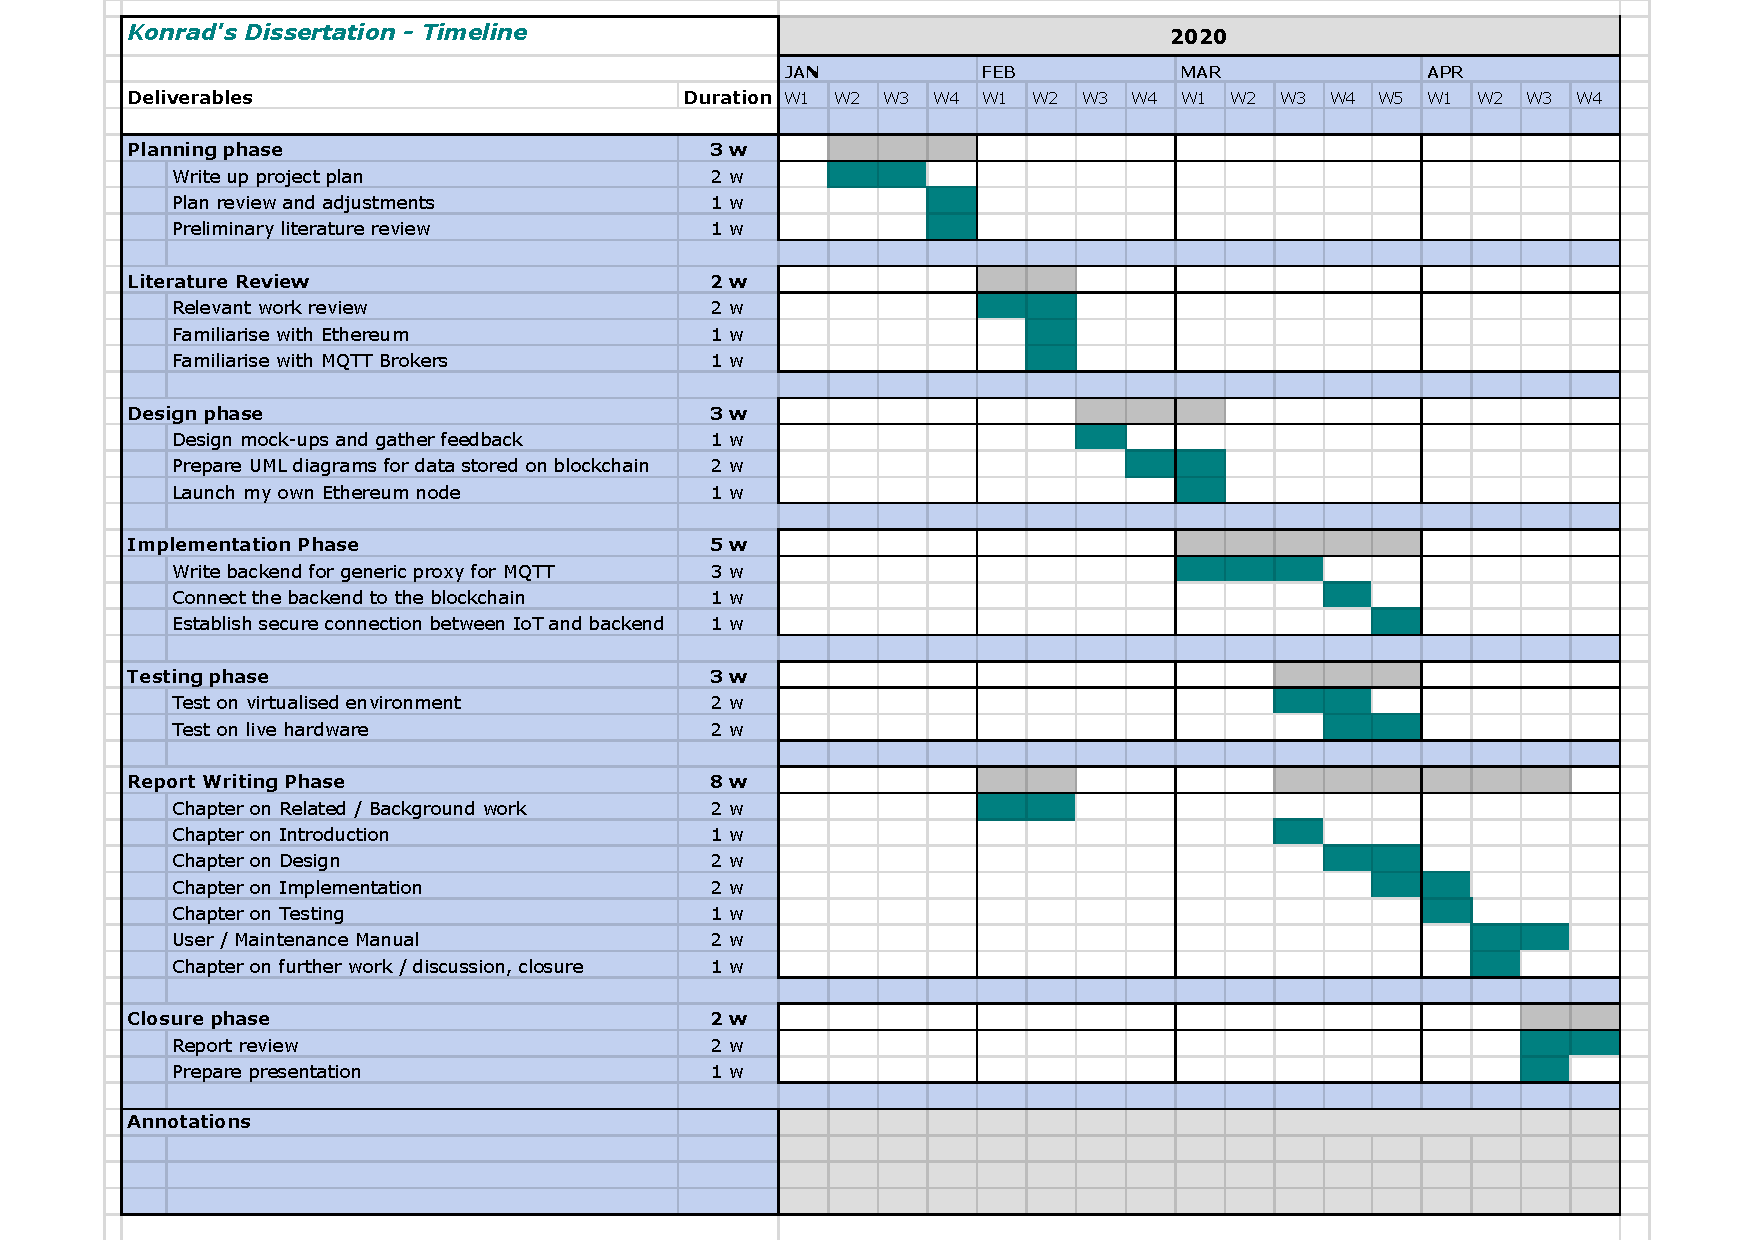
\includegraphics[scale=0.52]{timeline}}
\end{figure}
\pagebreak

\bibliography{ProjectPlan}

\end{document}
